\documentclass[10pt,a4paper]{article}
\usepackage[utf8]{inputenc}
\usepackage[italian]{babel}
\usepackage{amsmath}
\usepackage{amsfonts}
\usepackage{amssymb}
\usepackage{graphicx}
\usepackage{gensymb}
\usepackage[left=2cm,right=2cm,top=2cm,bottom=2cm]{geometry}
\newcommand{\rem}[1]{[\emph{#1}]}

\author{Gruppo BN \\ Federico Belliardo, Marco Costa, Lisa Bedini}
\title{Ottica 1}
\begin{document}

\maketitle
\section{Scopo dell'esperienza}
Questa esperienza si divide in due parti: A e B.
La parte A è dedicata al calcolo della lunghezza d'onda del sodio, mentre la parte B sfrutta la luce emessa da tre lampade diverse per calcolare la costante di Rydberg e la risoluzione dello spettroscopio a reticolo.\\

\section{Materiale occorrente}
\begin{itemize}
\item lampada al cadmio;
\item lampada al sodio;
\item lampada al mercurio;
\item lampada a idrogeno;
\item elemento dispersivo A: prisma;
\item elemento dispersivo B: reticolo;
\item supporto con goniometro integrato;
\end{itemize}
Inoltre avremo a disposizione due telescopi, uno di raccolta della luce dotato di fenditura per regolare l'intensità del fascio, e uno di osservazione solidale a un supporto mobile dotato di goniometro, per misurare la posizione del telescopio rispetto all'elemento dispersivo.\\
\section{Parte A - Descrizione esperimento}
\subparagraph{Lampada al cadmio}
Per tarare l'apparato strumentale si è posta la lampada al cadmio in modo da allineare le fenditure, della lampada stessa e del telescopio di raccolta. Abbiamo regolato l'apertura del diaframma al minimo così da avere l'incertezza minima, quindi abbiamo posizionando l'elemento dispersivo con un angolo di almeno $60\degree$ rispetto alla direzione del telescopio di raccolta e osservato le righe di emissione del cadmio, di colori rosso, verde, azzurro e viola. Come ultima cosa abbiamo ruotato lentamente il prisma per trovare l'angolo di minima dispersione per la riga verde \footnote{Perché ha la lunghezza d'onda più vicina a quella del sodio.}, cioè l'angolo di inversione del moto delle righe dello spettro che si osserva muovendo il prisma. Non abbiamo eseguito una misura dell'angolo $alpha_0$ al quale viene focalizzato il fascio (come sarà invece eseguito nella prossima parte) poiché risulta essere una costante additiva inessenziale nella nostra analisi dati.
Si è dunque eseguita la calibrazione spettrale, nota le lunghezze d'onda delle principali righe di emissione del cadmio. Abbiamo misurato l'angolo di osservazione di ciascuna riga (vedi tabella \ref{cadmio}) e eseguito un fit lineare $y=ax+b$ nel grafico $\alpha\, \textit{vs}\, 1/\lambda$ ottenendo come parametri $a = -3250 \pm 40 \frac{\degree}{nm}$ e $ b = 148.1 \pm 0.1 \degree$ e $\chi^2=23/2$. Il $\chi^2$ ottenuto è alto a causa del fatto che la curva di calibrazione lineare in funzione di $\frac{1}{\lambda}$ è solo un'approssimazione, in realtà si ha comportamento molto più complesso per il prisma. I dati raccolti si trovano in tabella \ref{cadmio} mentre in figura \ref{pin} è presente il grafico con il \emph{fit}.

\begin{table}[!htb]
\centering
\begin{tabular}{|c|c|c|}
\hline 
Colore & $\lambda (nm)$ & $\alpha (\degree)$ \\
\hline
Rosso & $643.8\pm0.1$ & $143 \degree 1' \pm 1'$ \\ 
\hline 
Verde & $508.643 \pm 0.001$ & $141 \degree 45' \pm 1'$ \\ 
\hline 
Azzurro & $480.0 \pm 0.1$ & $141 \degree 19' \pm 1'$ \\ 
\hline 
Viola & $467.8 \pm 0.1$	& $141 \degree 5' \pm 1'$ \\ 
\hline 
\end{tabular} 
\caption{Righe di emissione del cadmio con relativa posizione angolare.}\label{cadmio}
\end[table}

\begin{figure}[!htb]
  \centering
  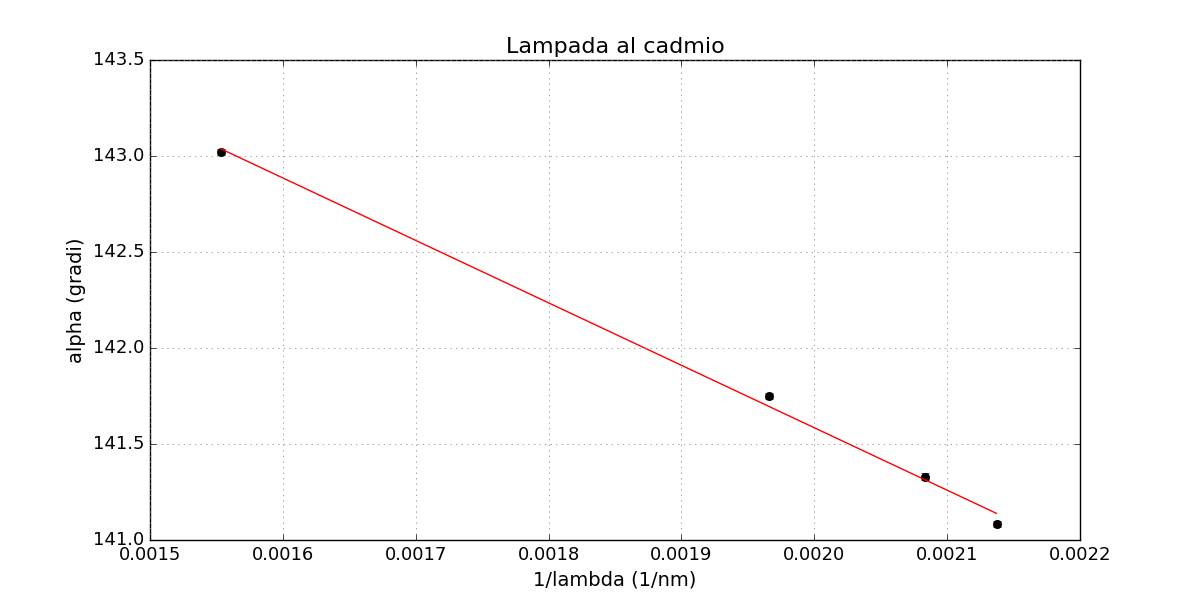
\includegraphics[scale=0.5]{imm.png}
\caption{Grafico $\alpha\, \textit{vs}\, 1/\lambda$ e \emph{fit}.}
\label{pin}
\end{figure}

Per eseguire i fit di tutta la relazione si è la funzione \emph{curvefit} della libreria \emph{pylab} con l'opzione \emph{$absolute\,sigma = "true"$}.\\

\subparagraph{Lampada al sodio}
Si è sostituita la lampada al cadmio con la lampada al sodio precedentemente accesa in modo che si stabilizzasse. Abbiamo individuato la riga\footnote{Un doppietto in realtà ma l'uso del prisma non consente tale risoluzione.} di emissione del sodio e misurata la sua posizione angolare, che risulta $\alpha_{Na}=142 \degree 35'\pm 1'$ \footnote{In tutta la relazione ogni misura angolare è intesa come media delle tre misure eseguite dai tre componenti del gruppo ed è intesa avere come errore quello di lettura sulla scala graduata del nonio.}. Usando le relazioni ricavate precedentemente dal \emph{fit}, si calcola $\lambda_{Na}=590 \pm 10 nm$. Questo valore sarà confrontato con quello ottenuto usando il reticolo, elemento dispersivo con più potere risolutivo del prisma.

\section{Parte B - Descrizione esperimento}
\subparagraph{Lampada al mercurio}
Si è rimosso il reticolo, quindi abbiamo iniziato la procedura per la taratura dell'apparato sperimentale. Abbiamo posto la lampada al mercurio e i telescopi in modo da allineare il sistema, successivamente abbiamo regolato l'ampiezza della fenditura e il fuoco dei telescopi. In queste condizioni si misura un angolo $\alpha_0 = 169 \degree 45 '\pm 1'$. D'ora in avanti tutte le misure di angoli saranno riportate come $\alpha=\alpha_{lettura}-\alpha_0$. Abbiamo posto il reticolo con un angolo di almeno $60\degree$ rispetto al telescopio di raccolta, quindi abbiamo controllato che le righe di interesse, quelle della serie di Balmer, fossero ben visibili.
Come ultima operazione si è calcolato il passo reticolare $d$. Per fare ciò abbiamo misurato l'angolo di ordine zero della riga verde e l'angolo della stessa riga al primo ordine, i due risultati sono: $\alpha_V^{0} = 58 \degree 8 ' \pm 2'$ e $\alpha_V^{1} = 106 \degree 7' \pm 2'$. Da semplici considerazioni geometriche si ricavano le seguenti relazioni:
\begin{equation}
\theta_i=\frac{1}{2}(\pi-\alpha_V^{0})=61\degree 56'\pm2'
\end{equation}
\begin{equation}
\theta_d=\pi-\theta_i-\alpha_1= 12 \degree 56' \pm 3
\end{equation}
Quindi è possibile calcolare $d$ sfruttando la relazione del reticolo 
\begin{equation}
d(sin{\theta_i}-sin{\theta_d})=m\lambda
\end{equation}
Si ottiene $d = 840.2 \pm 0.5 nm$. Considerando nota la lunghezza d'onda del mercurio $\lambda_{Hg}=546.074\pm0.001\,nm$ si calcola il numero di righe per millimetro $N = 1190 \pm 3$, in accordo con il valore nominale di 1200.

\subparagraph{Lampada a idrogeno}
Si è sostituita la lampada a mercurio con quella a idrogeno, in modo da avere la massima intensità per l'ordine zero senza modificare le distanze focali. Abbiamo quindi misurato la distanza angolare delle righe di emissione per calcolarne le lunghezze d'onda mediante la formula $d(\sin{\theta_i}-\sin{\theta_d})=m\lambda$. I risultati sono riportati in tabella \ref{idrogeno}. La riga verde non fa parte dello spettro dell'idrogeno e l'ultimo dato si riferisce alla riga viola del secondo ordine, pertanto i dati relativi a queste righe non saranno necessari nell'analisi dati, ma sono riportati nella tabella per completezza.\\

\begin{table}[!htb]
\centering
\begin{tabular}{|c|c|c|}
\hline
Colore & $\alpha$ ($\degree$) & $\lambda$ (nm)\\
\hline 
Viola & $98 \degree 2' \pm 1'$ & $432 \pm 2 nm$ \\ 
\hline 
Azzurro & $101 \degree 53' \pm 1'$ & $486 \pm 2 nm$ \\ 
\hline 
Verde (deb.)& $105 \degree 5' \pm 1'$ & $531 \pm 2 nm$ \\ 
\hline 
Rossa & $113 \degree 30' \pm 1'$ & $653 \pm 1 nm$ \\ 
\hline 
%Viola (2° Ord.) & $113 \degree 35' \pm 1'$ & _ \\ 
%\hline 
\end{tabular} 
\caption{Dati misurati per la lampada a idrogeno.}\label{idrogeno}
\end{table}

Lo spettro dell'idrogeno è descritto dall'equazione di Rydberg:
\begin{equation}
\frac{1}{\lambda}=R \left( \frac{1}{n_{1}^2}-\frac{1}{n_{2}^2} \right)
\end{equation}

Per la serie di \emph{Balmer}, la più visibile, $n_1=2$; a questa serie appartengono la riga viola con $n_2=5$, quella azzurra con $n_2=4$ e quella rossa con $n_2=3$. Si è effettuato un fit lineare a un parametro ottenendo un valore per la costante di Rydberg pari a $R = 10.9 \pm 0.1 \frac{1}{\mu m}$ in accordo con il valore atteso pari a $R=10.968\, \frac{1}{\mu m}$, associato a questo fit abbiamo $\chi^2 = 0.44/1$. Nel fit si è esclusa la riga verde che non appartiene all'idrogeno ma è dovuta a impurità nella lampada (infatti è molto debole).\\

\begin{figure}[!htb]
  \centering
  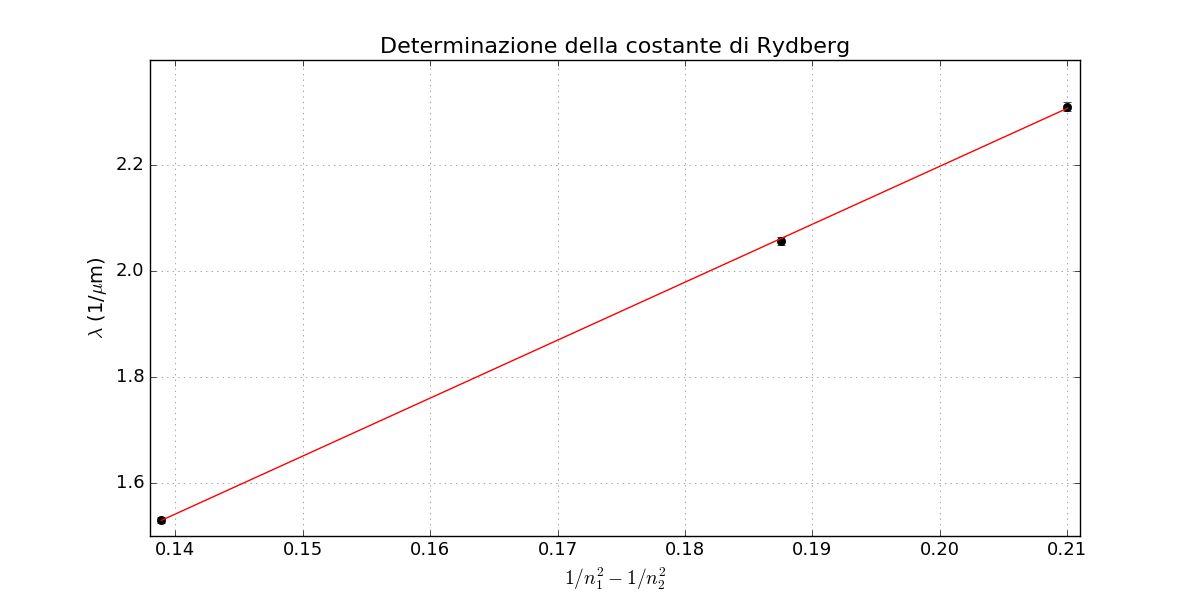
\includegraphics[scale=0.6]{ryd.png}
\caption{INSERIRE DIDASCALIA \emph{fit}.}
\label{pin}
\end{figure}


\subparagraph{Lampada al sodio}
Si è sostituita la lampada a idrogeno con quella al sodio per misurare la lunghezza d'onda del doppietto giallo e confrontare tale dato con quello attenuto nella prima parte dell'esperienza. Al primo ordine abbiamo misurato i seguenti valori angolari $\alpha_{Na,1}= 108\degree 42'\pm 1' $ e $\alpha_{Na,2}=108\degree 45' \pm 1'$, quindi, sfruttando l'equazione del reticolo si ottiene la lunghezza d'onda $\lambda_{Na,1}=583.0 \pm 2 nm$ e $\lambda_{Na,2}=583.0 \pm 2$.
Abbiamo abusato delle regole sulle cifre significative perché in tutta l'analisi dati gli errori sono sempre stati sovrastimati, ma si voleva mostrare la separazione tra le righe spettrali stimata di $0.8 \, nm$, contro quella attesa di $0.6 \, nm$, i due valori sono molto vicini.




\section{Conclusioni}
TUTTO BENE

\end{document}